\documentclass{essay}

\usepackage{graphicx}
\usepackage{amsmath,amssymb,mathtools}
\usepackage{cleveref}
\usepackage[binary-units=true]{siunitx}
\usepackage{csquotes}
\usepackage[backend=bibtex,style=numeric]{biblatex}
\addbibresource{bibliography.bib}
\renewcommand*{\bibfont}{\small\sffamily}

\sisetup{detect-family,detect-weight}

\title{Web malware detection with Markov random fields\\and belief propagation}
\author{\textbf{Matteo Dora} \enspace\textbullet\enspace matteo.dora@ens.fr}
\date{\today}

\begin{document}
\maketitle

\color{dark}
\sffamily

{\bfseries\sffamily\noindent As modern society has become increasingly dependent on digital techologies and communication networks, malicious software emerges as a major threat. Nefariously famous computer worms such as Code Red or Storm have caused economic losses estimated in the billions of USD \cite{karyotis_malware_2016}@todo(add references)and sophisticated state-sponsored attacks have leaked business secrets \cite{wp_sony_hack} or damaged military targets \cite{stuxnet}. Due to their increasing popularity, websites have become one of the most frequent attack vectors. Extensive research has been conducted to detect malicious web domains based on their behaviour \cite{zhauniarovich_survey_2018}. Here I follow a different approach, by analysing the topology of the interaction network between users and web domains, and I review a simple Markov random field (\textsc{MRF}) that allows to detect malicious domains and hosts, evaluating its predictive accuracy via numerical simulations.}

\section*{Introduction}

Malicious software has been around since the days of yore, but it is only in the last two decades that it became a highly profitable business. The massive amount of sensible information that is nowadays available on digital devices make for an attractive loot to cybercriminals, and the internet provides a very effective medium for propagation. With the profitability growth, more and more resources have been dedicated to malware development, leading to increasingly advanced tools. Modern malware can be roughly divided into two main categories. On one hand, criminal organisations and intelligence agencies sponsored the creation of highly sophisticated attack tools. Examples of this kind of malware are Stuxnet \cite{stuxnet}, a worm targeting Iran's nuclear infrastructure, and Zeus, a criminal botnet dismantled in 200x with more than 100 arrests worldwide @todo(add reference). On the other hand, older versions of advanced malware and lesser evoluted tools began circulating in a thriving black market, allowing small criminal groups and individuals to approach the business. These kind of malware is usually directed at novice users and diffuses through email, websites and social networks. In the following, I will focus on this latter category of less sophisticated but widely spread malware, altough some of the methods described may be used in more advanced contexts.

In the recent years, the most popular threat is represented by based malware \cite{liu_web_2017} @todo(add references). This breed of malware is injected into target devices by malicious web pages. It can spread by inducing users into following malicious hyperlinks, typically distributed via social networks or email. Other common attack vectors are legitimate websites compromised by means of malicious techniques such as cross site scripting (\textsc{xss}) or \textsc{sql} injection and configured to diffuse malware. Malicious web domains have usually a relatively short life, as once identified they can immediately taken down by authorities or blocked by antivirus software. Nonetheless, cybercriminals are continuously registering new malicious domains (or compromising existing ones), in an infinite hide-and-seek game. How can web threats be prevented? Is it possible to identify malicious domains at early stage, before most of the damage is done?

In the following, I will present a simple model for malware spreading based on Markov random fields. Then I will analyse the network topology on which the model can be applied in the case of web domains. Finally I will use an inference method, previously explored by Manadhata et al. \cite{manadhata_detecting}, and check with numerical simulations how well it performs in identifying malicious web domains.

\section*{Modelling malicious web domains}

Many approaches modelling malware epidemics have been proposed based on classical compartmental models such as \textsc{sis} and \textsc{sir} \cite{liu_web_2017,gil2014genetic,karyotis_malware_2016}. Although these deterministic models are valid and have proven successful (for example in the case of the Code Red worm \cite{zou_code}), they can only describe the global characteristics of the infection diffusion. Stochastic epidemic models would overcome most of the limitations of deterministic ones, but analytical analysis (e.g. using queuing theory) is often intractable. Moreover, both categories are extremely sensible to variations in the topology of the system, which can affect the system ergodicity, making these models an inconvenient choice when dealing with complex networks.

Following the framework proposed by Karyotis \cite{karyotis_malware_2016,karyotis2017markov}, here I will focus on a simpler model constituted by a Markov random field (\textsc{mrf}). A \textsc{mrf} is network of random variables interacting only with their neighbours. Despite their simplicity, \textsc{mrf}s are good candidates to describe a malware propagation. The Markov spatial property is a sensible assumption, as malware can only spread by direct contact. Also, they are extremely robust to topological variations, as each variable, given its neighbours, is conditionally independent of any other node. This latter characteristic make them very useful to model processes on different kind of networks.


To describe malware diffusion we consider the \textsc{SIS} paradigm and build a \textsc{mrf} where nodes can assume two states: susceptible ($x = +1$) or infected ($x = -1$). Nodes are organised on a network where links represent data exchange between the nodes. Intuitively, susceptible nodes communicating with infected neighbours will turn infected with higher probability. This kind of interaction can be described by an Ising Hamiltonian:
\begin{align}
& p\left(X\right) = \frac{1}{Z}e^{-\beta H\left(X\right)}\\
& H\left(X\right) = - J \sum_{\langle i, j\rangle} x_i x_j - \sum_i h_i x_i
\end{align}
where $X$ denotes a sequence of node states $(x_0, x_1, x_2, \dots)$ (the system configuration), $J$ is the interaction potential and $h_i$ is the local field of node $i$. It is important to notice that this joint probability function factorises:
\begin{align}
p\left(X\right) &= \frac{1}{Z} \left( \prod_{i} e^{\beta h_i x_i}\right) \left(\prod_{\langle i, j \rangle} e^{\beta J x_i x_j}\right) \\
          & \doteq \frac{1}{Z} \left(\prod_{i} \phi_i(x_i)\right) \left(\prod_{\langle i, j \rangle} \phi_ij(x_i, x_j)\right)
\end{align}
In this setting, all the nodes are in principle free to switch between the two states. Yet, we want to represent attackers as infected nodes that never change state. We can do that by setting their local field to infinite (in this case, $h_{attacker} = - \infty$). The same technique in the case we want to fix the state of susceptible nodes.
Finally, we add to this model a human factor. In fact, system administrators are usually checking their domains for malware and keep them healthy. Although history tells us that no domains are immune to malware \cite{krebs2006hacked}, administrators of popular domains will likely detect attacks and respond more quickly. To consider this in the model, we add to domain nodes a small positive field $h_i \sim log(d_i)$, where $d_i$ is the degree of node $i$.

\subsection*{Network topology}

\begin{figure}
  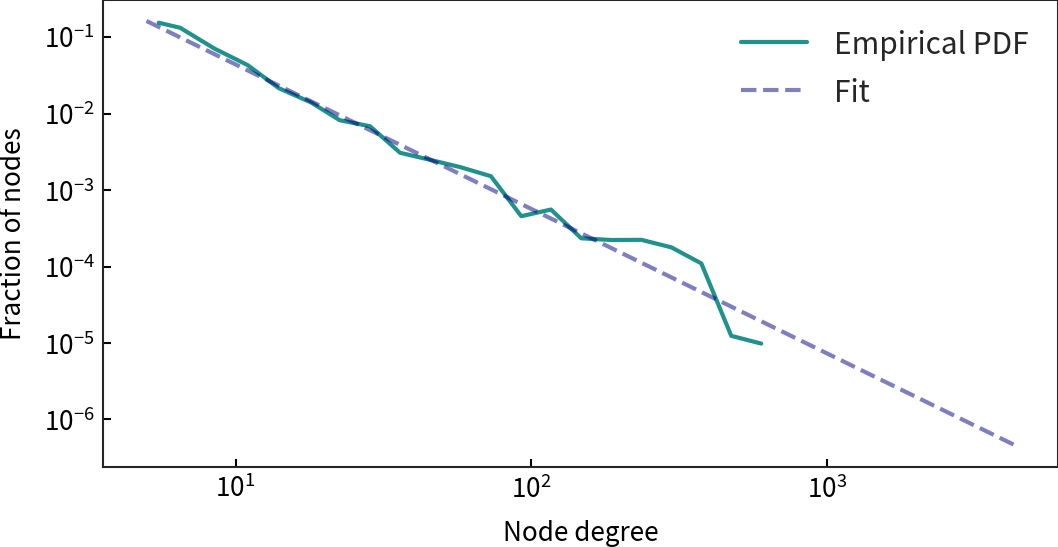
\includegraphics{fig/powerlaw.png}
  \caption{
    Degree distribution obtained by the analysis of the \textsc{ctu-13} dataset (log-log plot). The result is typical of a scale-free network, showing the characteristic power law degree distribution. A power law fit (dashed line) in the form $p(x) \sim x^{-\alpha}$ results in exponent $\alpha = 1.89$.
  }
  \figrule
  \label{fig:powerlaw}
\end{figure}

Let us suppose that, given a local network, we can intercept every request coming from local hosts and directed to domains in the outer web (e.g. through a \textsc{http} proxy, as described in \cite{manadhata_detecting}). Using this knowledge, we can build a bipartite graph linking local hosts to the remote domains they interact with. In a real network, these links will not be uniformly distributed, but will likely depend on the popularity of the domains. Which are the characteristics of the interaction network between users (local hosts) and web domains? It has been shown that when popularity drives the node connectivity (the so called \emph{preferential attachment} mechanism), a scale-free topology may emerge \cite{barabasi1999emergence,albert2002statistical}. Scale-free graphs are characterised by a power law node degree distribution. Examples are social networks, or the network of web pages connected by hyperlinks. To check whether the host-domain communicaton network belongs to this topological class, I analysed the \textsc{ctu-13} dataset provided by the Czech Technical University \cite{ctu13}. The \textsc{ctu-13} data contains the traffic flows between a local network and the outer internet. For privacy concerns, only a truncated version of \textsc{ip} packets is provided, so that information about the payload is lost. Nevertheless, it is possible to recover the traffic flow between \textsc{ip} addresses. I preprocessed the data by discarding the internal traffic flows (i.e. those between hosts of the local network) and considering only exchanges greater than \SI{500}{\byte} (a sensible minimum for a web page request through \textsc{http}).
A network is built by linking hosts and domain based on the flows in the dataset after preprocessing. I found that the empirical degree distribution of this network (\cref{fig:powerlaw}) is well described by a power law, confirming the initial hypothesis.

Based on this result, we can build host-domain communication graphs by growing a bipartite graph via preferential attachment \cite{albert2002statistical,ohkubo_generation_2005}. For this purpose, I adapted the Barábasi--Albert algorithm for the case of bipartite networks \cite{code}. We can thus generate arbitrary network strutures to test our model.



\begin{figure}
  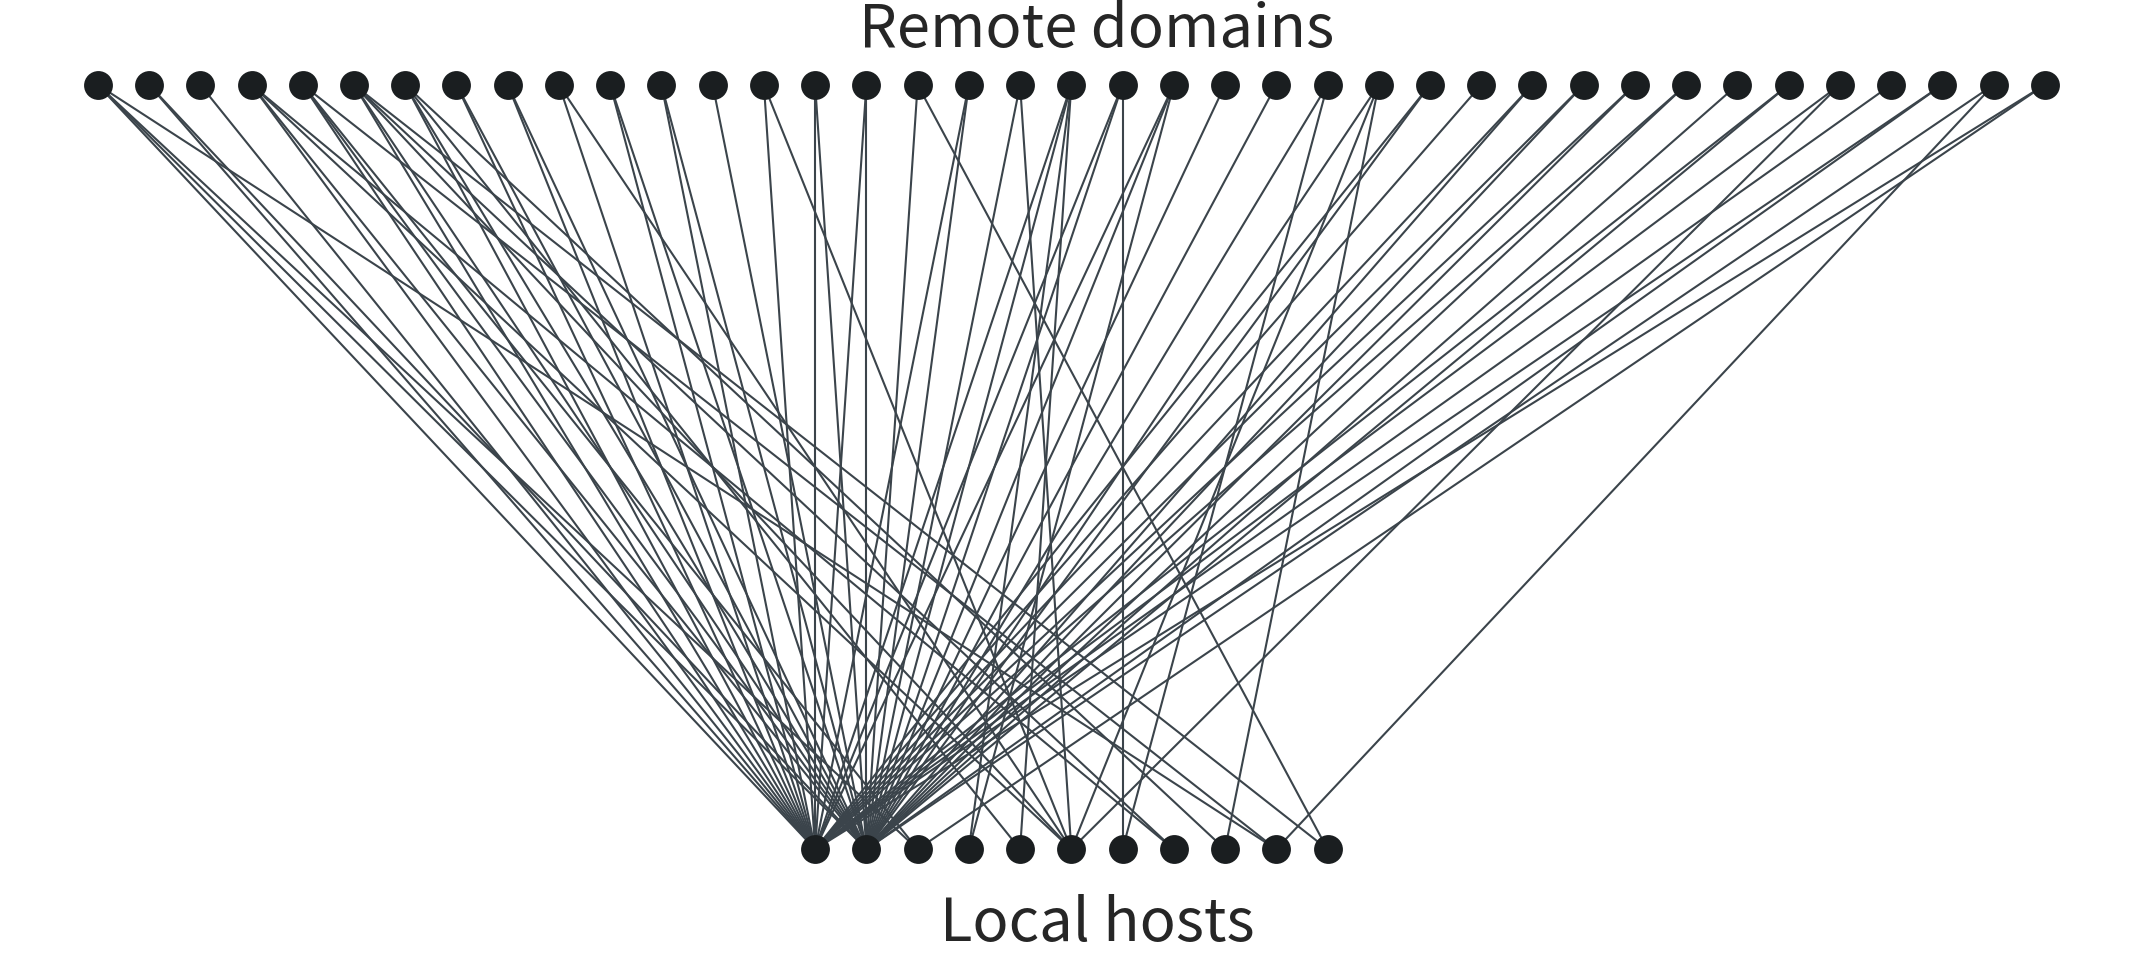
\includegraphics{fig/graph.png}
  \caption{
    Example of bipartite scale-free graph for hosts and domains. The graph was generated using the Barábasi--Albert algorithm \cite{albert2002statistical}, conveniently adapted for the case of bipartite networks.
    \figrule
  }
  \label{fig:g_a}
\end{figure}

\section*{Detecting malicious actors}

Let us assume that we can inspect the state of some of the hosts in the local network. Is it possible, given this partial knowledge, to identify malicious web domains? A known method to perform this kind of inference is belief propagation. This algorithm, initially proposed by Pearl for trees \cite{pearl1982reverend} and polytrees \cite{pearl2014probabilistic}, can be used to estimate the marginal probability of hidden variables (given the known variables) in an arbitrary Markov random field. Belief propagation is a message-passing algorithm, where each node send to neighbours its estimate of their states (belief) in form of a \emph{message}, and subsequently collects messages from neighbours to update its own belief. Usually, after a sufficient number of iterations the beliefs converge to an approximate estimate of marginals, although this cannot be proved in general.

I implemented a specific version of belief propagation known as max-product message passing, where the message from node $i$ to its neighbour $j$ is defined as:
\begin{equation}
  m_{i \to j}\left(x_i\right) = \max_{x_i = \pm 1}
  \left\{
    \phi_{ij}(x_i, x_j) \phi_i(x_i) \smashoperator{\prod_{k \in \mathcal{N}(i)\setminus j}} m_{k \to i}(x_i)
  \right\}
\end{equation}
and the belief assigned to the state $x_i$ at node $i$ is
\begin{equation}
  b(x_i) = \phi_i(x_i) \smashoperator{\prod_{k \in \mathcal{N}(i)}} m_{k \to i}(x_i)
\end{equation}
It must be noted that in this case the belief does not correspond to the marginal distribution, but can be considered a score function. The prediction for node $i$ will be the state that maximises the score. Detailed implementation of the belief propagation algorithm can be found in the supporting code \cite{code}.

\subsection*{Prediction accuracy}

To evaluate the quality of predictions I ran numerical simulations. First, I generated configurations for the model using Markov chain Monte Carlo (\textsc{mcmc}) on random bipartite scale-free networks. The networks were generated using the Barábasi--Albert algorithm, as described in the previous section, with 1500 total nodes comprising @ local hosts. A small number of malicious domains were fixed in the system. To improve the efficacy of the \textsc{mcmc} algorithm, I used simulated annealing (\textsc{sa}), decreasing temperature as $\beta \sim \log t$, where $t$ is the simulation time. Then, I generated a prediction on the domain states given a variable number of known hosts using belief propagation. Following the intuition that popular domains represent a more tough target for malware, a prior was set on the top 50 most popular domains with a logistic function mapping their popularity to an increasing probability of being in the non-infected state (a similar approach was proposed in \cite{manadhata_detecting}). Accuracy was defined as the fraction of correct predictions over the total number of domains.

\section*{Conclusions}


\vfill
% \nocite{*}
\printbibliography

\end{document}
